\section{Data and Results}

\subsection{Monogram frequency}
Monogram frequency counts are most effective on substitution type ciphers such as the caesar cipher, substitution cipher, polybius square etc. It works because any natural language text follows a very specific frequency distribution, which is not masked by substitution ciphers\cite{text_characterisation}.

\selectlanguage{ethiop}
\begin{table}[h!]
    \begin{center}
        \begin{tabular}{|| r | l | r | r ||}
            \hline
            \foreignlanguage{english}{Rank} & 
            \foreignlanguage{english}{Character} &
            \foreignlanguage{english}{Count} & 
            \foreignlanguage{english}{Percentage} \\
            \hline
            \hline
            1 & n & 738643 & 4.28079 \\
            2 & t & 680710 & 3.94504 \\
            3 & ya & 638802 & 3.70216 \\
            4 & ba & 566363 & 3.28234 \\
            5 & ma & 556450 & 3.22489 \\
            6 & r & 455960 & 2.64251 \\
            7 & w & 436064 & 2.5272 \\
            8 & ta & 427311 & 2.47647 \\
            9 & s & 387069 & 2.24325 \\
            10 & nA & 347901 & 2.01625 \\
            11 & yA & 331325 & 1.92018 \\
            12 & m & 321078 & 1.8608 \\
            13 & 'e & 301741 & 1.74873 \\
            14 & : & 294046 & 1.70413 \\
            15 & 'a & 287540 & 1.66643 \\
            16 & y & 273357 & 1.58423 \\
            17 & ^c & 271122 & 1.57128 \\
            18 & g & 269841 & 1.56386 \\
            19 & ga & 265020 & 1.53592 \\
            20 & ka & 258721 & 1.49941 \\
            21 & ra & 251049 & 1.45495 \\
            22 & mA & 245490 & 1.42273 \\
            23 & l & 244525 & 1.41714  \\
            \hline
        \end{tabular}
    
        \selectlanguage{english}
        \caption{Top 23 - Monogram frequency}
        \label{table:1}
    \end{center}
\end{table}

\selectlanguage{english}
\begin{figure}[H]
    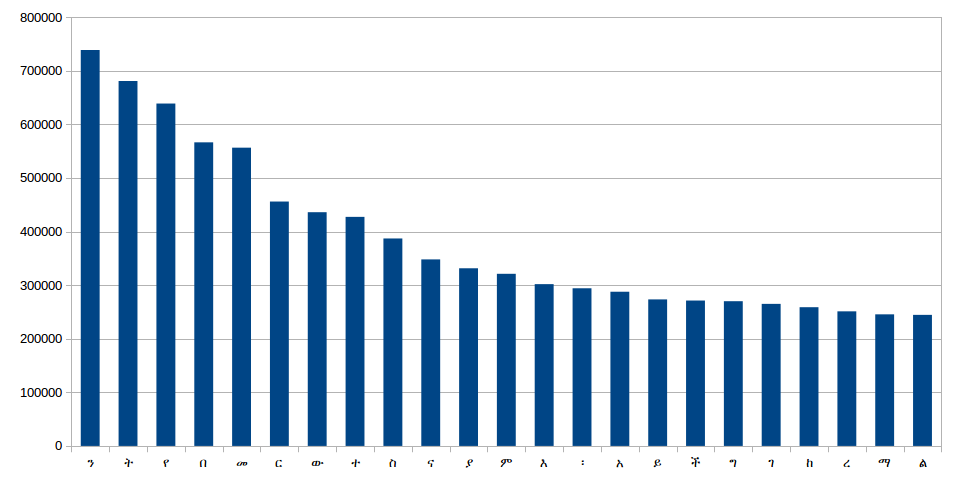
\includegraphics[width=0.48\textwidth]{fig_top23_letters}
    \centering
    \caption{Top 23 - Monogram frequency}
    \label{fig:mesh1}
\end{figure}

\subsection{Bigram frequency}
Bigram counts maintain the same principle as monogram counts, but instead of counting occurrences of single characters, bigram counts count the frequency of pairs of characters\cite{text_characterisation}.

\selectlanguage{ethiop}
\begin{table}[H]
    \begin{center}
        \begin{tabular}{|| r | l | r || r | l | r ||}
        \hline
        \foreignlanguage{english}{ } &
        \foreignlanguage{english}{Character} & 
        \foreignlanguage{english}{Count} & 
        \foreignlanguage{english}{ } &
        \foreignlanguage{english}{Character} &
        \foreignlanguage{english}{Count} \\
        \hline
        \hline
            1 & 'ene & 93271 & 11 & bama & 48123 \\
            2 & yami & 87682 & 12 & wene & 47487 \\
            3 & yata & 80939 & 13 & bata & 46551 \\
            4 & ^cawe & 78480 & 14 & nate & 44970 \\
            5 & wo^ce & 74229 & 15 & bate & 41547 \\
            6 & :: & 71312 & 16 & rate & 40688 \\
            7 & to^ce & 54518 & 17 & kata & 38304 \\
            8 & honu & 54498 & 18 & mane & 37955 \\
            9 & maho & 52918 & 19 & ^cene & 36395 \\
            10 & 'enA & 50904 & 20 & yama & 36001 \\
        \hline
        \end{tabular}
        
        \selectlanguage{english}
        \caption{Top 20 - Bigram frequency}
        \label{table:2}
    \end{center}
\end{table}

\selectlanguage{english}
\begin{figure}[H]
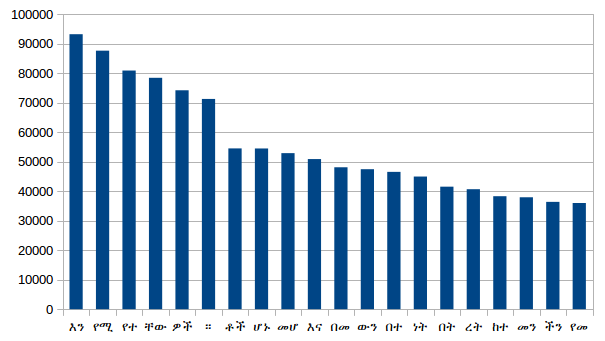
\includegraphics[width=0.5\textwidth]{fig_top20_digraph}
\centering
\end{figure}

\subsection{Trigram frequency}
Just as bigram counts count the frequency of pairs of characters, trigram counts count the frequency of triple characters\cite{text_characterisation}.

\selectlanguage{ethiop}
\begin{table}[H]
    \begin{center}
        \begin{tabular}{|| r | l | r || r | l | r ||}
            \hline
            \foreignlanguage{english}{ } &
            \foreignlanguage{english}{Character} &
            \foreignlanguage{english}{Count} &
            \foreignlanguage{english}{ } &
            \foreignlanguage{english}{Character} &
            \foreignlanguage{english}{Count} \\
            \hline
            \hline
                1 & mahonu & 46465 & 11 & yo.peyA & 16220   \\
                2 & le:: & 25242 & 12 & teyo.pe & 16074     \\
                3 & 'enedi & 25239 & 13 & masara & 15673    \\
                4 & lE:: & 24421 & 14 & bEto^ce & 15665     \\
                5 & 'enedu & 22040 & 15 & 'iteyo & 15617    \\
                6 & 'egezi & 21588 & 16 & hisAbe & 15541    \\
                7 & yamiyA & 20648 & 17 & minise & 15304    \\
                8 & wese^Ce & 18908 & 18 & honune & 14916   \\
                9 & manege & 18554 & 19 & ba^gate & 14504   \\
                10 & ^cawene & 16357 & 20 & 'eneda & 14436  \\
            \hline
        \end{tabular}
    
        \selectlanguage{english}
        \caption{Top 20 - Trigram frequency}
        \label{table:3}
    \end{center}
\end{table}

\selectlanguage{english}
\begin{figure}[H]
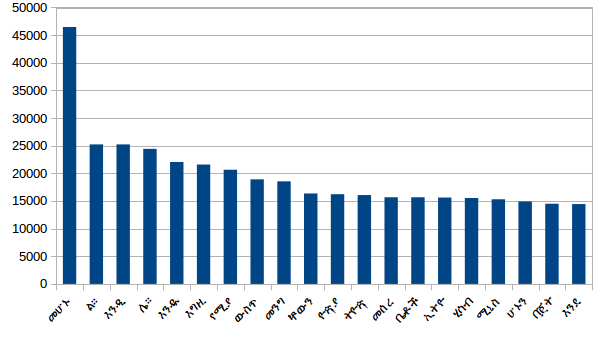
\includegraphics[width=0.5\textwidth]{fig_top20_trigraph}
\centering
\end{figure}

\subsection{Consonant group ('\foreignlanguage{ethiop}{bEte}') frequency}

Consonant group frequency is the frequency of the 34 Amharic consonant variants which is one row from the Ge`ez script consonants cluster. All of the '\foreignlanguage{ethiop}{ha}', '\foreignlanguage{ethiop}{hu}', '\foreignlanguage{ethiop}{hi}', '\foreignlanguage{ethiop}{hA}' ... variants are grouped together and analyzed\cite{ethiopic_scripts}. 

\selectlanguage{ethiop}
\begin{table}[H]
    \begin{center}
        \begin{tabular}{|| r | l | r || r | l | r ||}
        \hline
        \foreignlanguage{english}{ } &
        \foreignlanguage{english}{Character} &
        \foreignlanguage{english}{Count} &
        \foreignlanguage{english}{ } &
        \foreignlanguage{english}{Character} &
        \foreignlanguage{english}{Count} \\
        \hline
        \hline
            1 & ta & 1502138 & 11 & 'a & 698619 \\
            2 & na & 1462331 & 12 & da & 640813 \\
            3 & ya & 1408562 & 13 & ka & 598522 \\
            4 & ma & 1382417 & 14 & ha & 497119 \\
            5 & ba & 1170744 & 15 & ^ca & 408120 \\
            6 & ra & 1131021 & 16 & qa & 386470 \\
            7 & la & 967577 & 17 & ^Ca & 375543 \\
            8 & wa & 844325 & 18 & fa & 277775 \\
            9 & sa & 759615 & 19 & za & 261978 \\
            10 & ga & 736809 & 20 & ^ga & 182281 \\
        \hline
        \end{tabular}
    
        \selectlanguage{english}
        \caption{Consonant group ('\foreignlanguage{ethiop}{bEte}') frequency}
        \label{table:4}
    \end{center}
\end{table}

\begin{figure}[H]
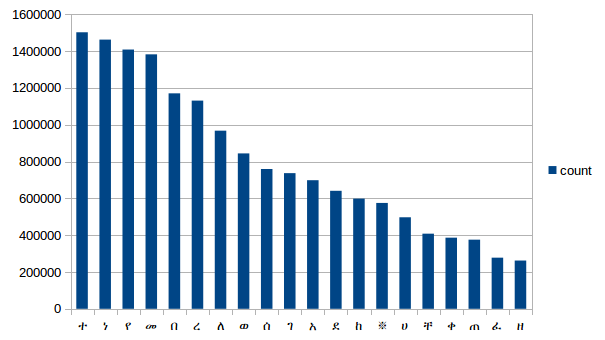
\includegraphics[width=0.48\textwidth]{fig_top20_bet-graph}
\centering
\end{figure}

\begin{figure}[H]
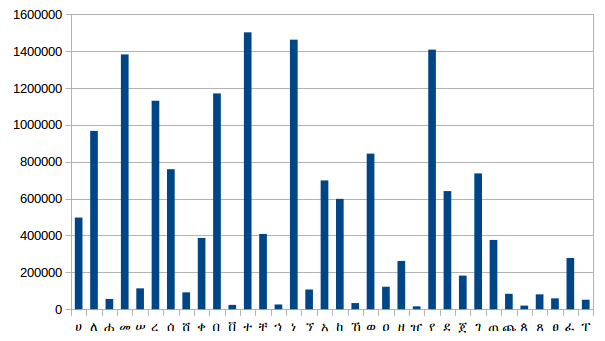
\includegraphics[width=0.48\textwidth]{fig_all_bet-graph}
\centering
\end{figure}

\selectlanguage{english}

\subsection{Vowel group ('\foreignlanguage{ethiop}{madabe}') frequency}
Vowel group frequency is the frequency of the vowel variants which will modify each consonant (i.e one column from the Ge`ez script consonants cluster). All of the '\foreignlanguage{ethiop}{sAdese}' variants ('\foreignlanguage{ethiop}{he}', '\foreignlanguage{ethiop}{le}', '\foreignlanguage{ethiop}{.he}', '\foreignlanguage{ethiop}{me}' ... ) are grouped together and analyzed\cite{ethiopic_scripts}.

\selectlanguage{ethiop}
\begin{table}[H]
    \begin{center}
        \begin{tabular}{|| r | r | l | r ||}
        \hline
        \foreignlanguage{english}{} & 
        \foreignlanguage{english}{Character} & 
        \foreignlanguage{ethiop}{madabe} & 
        \foreignlanguage{english}{Count} \\
        \hline
        \hline
        1 & 6 & \foreignlanguage{ethiop}{sAdese} & 5848229 \\
        2 & 1 & \foreignlanguage{ethiop}{ge`eze} & 4933207 \\
        3 & 4 & \foreignlanguage{ethiop}{rAbe`e} & 2661791 \\
        4 & 2 & \foreignlanguage{ethiop}{kA`ebe} & 1046439 \\
        5 & 3 & \foreignlanguage{ethiop}{'sAlese} & 1044916 \\
        6 & 7 & \foreignlanguage{ethiop}{sAbe`e} & 720252 \\
        7 & 5 & \foreignlanguage{ethiop}{_hAmese} & 680979 \\
        8 & 8 & \foreignlanguage{ethiop}{zamada rAbe`e} & 318991 \\
        \hline
        \end{tabular}
        
        \selectlanguage{english}
        \caption{Top 20 - Vowel group ('\foreignlanguage{ethiop}{madabe}') frequency}
        \label{table:5}
    \end{center}
\end{table}

\selectlanguage{english}
\begin{figure}[H]
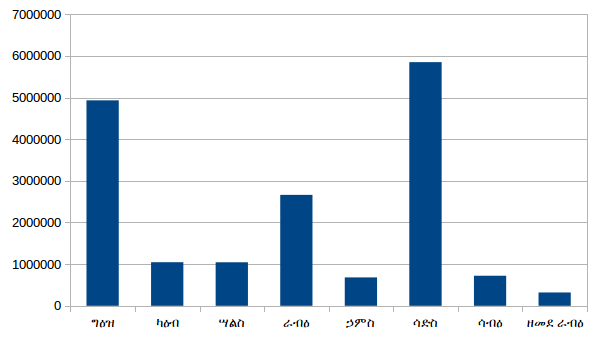
\includegraphics[width=0.48\textwidth]{charts/fig_all_medeb-graph}
\centering
\end{figure}

\subsection{Double letter frequency}
A double-letter word is one that contains consecutive letters that are the same, such as rabbit, deer or kitten. For each letter of the alphabet, this are the most common double letters in Amharic.

\selectlanguage{ethiop}
\begin{table}[H]
    \begin{center}
    \begin{tabular}{|| r | l | r || r | l | r ||}
    \hline
    \foreignlanguage{english}{ } & 
    \foreignlanguage{english}{Character} &
    \foreignlanguage{english}{Count} &
    \foreignlanguage{english}{ } & 
    \foreignlanguage{english}{Character} &
    \foreignlanguage{english}{Count} \\
    \hline
    \hline
    1 & : & 71312 & 11 & me & 3091 \\
    2 & ma & 17992 & 12 & le & 3056 \\
    3 & ^sA & 9540 & 13 & lE & 2362 \\
    4 & te & 8785 & 14 & we & 2031 \\
    5 & ne & 6474 & 15 & nA & 1925 \\
    6 & yA & 6255 & 16 & sA & 1891 \\
    7 & ^Ce & 6024 & 17 & ^CA & 1867 \\
    8 & ke & 5975 & 18 & tA & 1836 \\
    9 & ba & 4090 & 19 & ta & 1701 \\
    10 & qua & 3769 & 20 & lA & 1616 \\
    \hline
    \end{tabular}
    
    \selectlanguage{english}
    \caption{Top 20 - Double letter frequency}
    \label{table:6}
    \end{center}
\end{table}

\selectlanguage{english}
\begin{figure}[H]
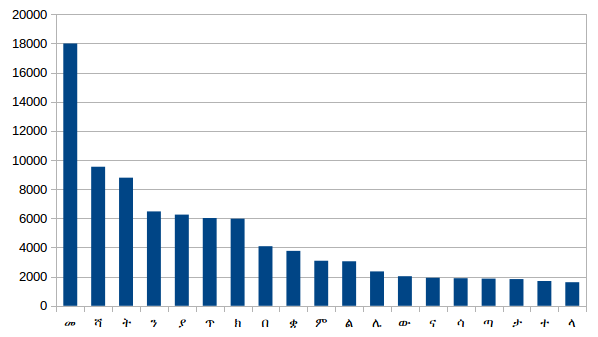
\includegraphics[width=0.48\textwidth]{charts/fig_all_double_letter-graph}
\centering
\end{figure}

\subsection{First letter frequency}
First letter frequency is the frequency of a given Amharic language first letter from a given word. 

\selectlanguage{ethiop}
\begin{table}[H]
    \begin{center}
    \begin{tabular}{|| r | l | r || r | l | r ||}
    \hline
    \foreignlanguage{english}{ } & 
    \foreignlanguage{english}{Character} &
    \foreignlanguage{english}{Count} &
    \foreignlanguage{english}{ } & 
    \foreignlanguage{english}{Character} &
    \foreignlanguage{english}{Count} \\
    \hline
    \hline
    1 & ya & 569324 & 11 & yA & 72231 \\
    2 & ba & 414816 & 12 & la & 71432 \\
    3 & ma & 259743 & 13 & se & 66667 \\
    4 & 'e & 238565 & 14 & ge & 48456 \\
    5 & 'a & 208080 & 15 & we & 42183 \\
    6 & ka & 121484 & 16 & me & 42005 \\
    7 & ta & 117446 & 17 & ke & 41459 \\
    8 & wa & 85590 & 18 & bA & 41416 \\
    9 & mA & 78348 & 19 & be & 40596 \\
    10 & ye & 72597 & 20 & li & 38199 \\
    \hline
    \end{tabular}
    
    \selectlanguage{english}
    \caption{Top 20 - First letter frequency}
    \label{table:7}
    \end{center}
\end{table}

\selectlanguage{english}
\begin{figure}[H]
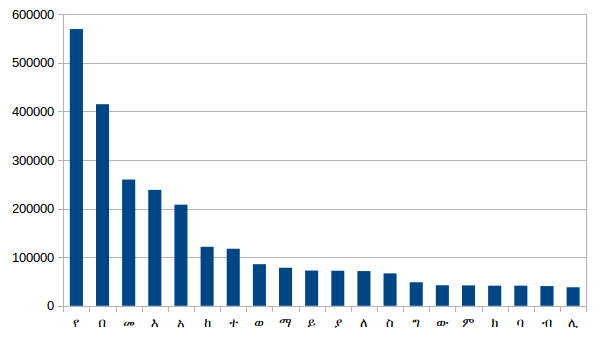
\includegraphics[width=0.48\textwidth]{charts/fig_all_first_letter-graph}
\centering
\end{figure}

\subsection{Second letter frequency}
Second letter frequency is the frequency of a given Amharic language second letter from a given word. 

\selectlanguage{ethiop}
\begin{table}[H]
    \begin{center}
    \begin{tabular}{|| r | l | r || r | l | r ||}
    \hline
    \foreignlanguage{english}{ } & 
    \foreignlanguage{english}{Character} &
    \foreignlanguage{english}{Count} &
    \foreignlanguage{english}{ } & 
    \foreignlanguage{english}{Character} &
    \foreignlanguage{english}{Count} \\
    \hline
    \hline
    1 & ne & 211523 & 11 & nA & 74411 \\
    2 & ma & 171288 & 12 & la & 68440 \\
    3 & ta & 147704 & 13 & ho & 66992 \\
    4 & re & 129813 & 14 & be & 59655 \\
    5 & mi & 124359 & 15 & me & 57804 \\
    6 & se & 113693 & 16 & sa & 53831 \\
    7 & mA & 95597 & 17 & le & 52029 \\
    8 & ye & 93176 & 18 & 'a & 51903 \\
    9 & ga & 82967 & 19 & we & 51116 \\
    10 & ge & 78444 & 20 & rA & 49058 \\
    \hline
    \end{tabular}
    
    \selectlanguage{english}
    \caption{Top 20 - Second letter frequency}
    \label{table:8}
    \end{center}
\end{table}

\selectlanguage{english}
\begin{figure}[H]
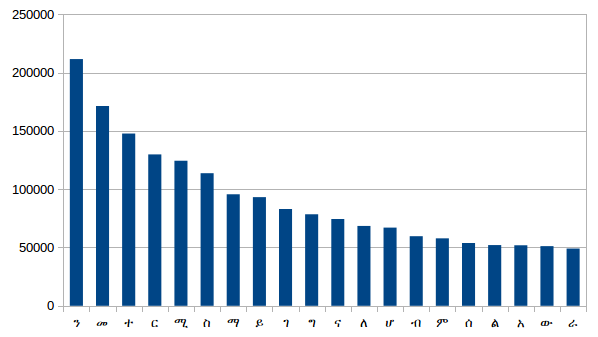
\includegraphics[width=0.48\textwidth]{charts/fig_all_second_letter-graph}
\centering
\end{figure}

\subsection{Last letter frequency}
Last letter frequency is the frequency of a given Amharic language last letter from a given word. 


\selectlanguage{ethiop}
\begin{table}[H]
    \begin{center}
    \begin{tabular}{|| r | l | r || r | l | r ||}
    \hline
    \foreignlanguage{english}{ } & 
    \foreignlanguage{english}{Character} &
    \foreignlanguage{english}{Count} &
    \foreignlanguage{english}{ } & 
    \foreignlanguage{english}{Character} &
    \foreignlanguage{english}{Count} \\
    \hline
    \hline
    1 & te & 467777 & 11 & ye & 75082 \\
    2 & ne & 273331 & 12 & ; & 69485 \\
    3 & nA & 247121 & 13 & be & 65238 \\
    4 & : & 212763 & 14 & le & 64701 \\
    5 & we & 208305 & 15 & tu & 63441 \\
    6 & re & 190347 & 16 & :: & 59351 \\
    7 & ^ce & 156041 & 17 & se & 56831 \\
    8 & me & 138486 & 18 & lE & 51317 \\
    9 & , & 88674 & 19 & rA & 51164 \\
    10 & yA & 82511 & 20 & := & 50495 \\
    \hline
    \end{tabular}
    
    \selectlanguage{english}
    \caption{Top 20 - Last letter frequency}
    \label{table:9}
    \end{center}
\end{table}

\selectlanguage{english}
\begin{figure}[H]
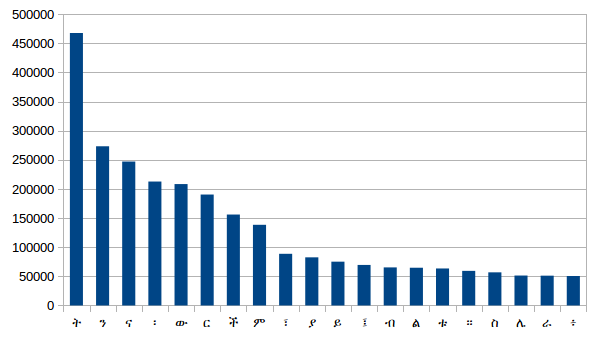
\includegraphics[width=0.48\textwidth]{charts/fig_all_last_letter-graph}
\centering
\end{figure}

\subsection{Word length frequency}
The frequency of the Amharic language words length statistics. 
\begin{table}[H]
    \begin{center}
    \begin{tabular}{|| r | l | r ||}
    \hline
    \foreignlanguage{english}{ } & 
    \foreignlanguage{english}{Length} &
    \foreignlanguage{english}{Count} \\
    \hline
    \hline
    1 & 4 & 928666 \\
    2 & 3 & 787376 \\
    3 & 5 & 701324 \\
    4 & 6 & 437831 \\
    5 & 2 & 367253 \\
    6 & 7 & 170080 \\
    7 & 8 & 69592 \\
    8 & 9 & 21743 \\
    9 & 1 & 16734 \\
    10 & 10 & 5602 \\
    \hline
    \end{tabular}
    
    \selectlanguage{english}
    \caption{Top 20 - Word length frequency}
    \label{table:10}
    \end{center}
\end{table}

\selectlanguage{english}
\begin{figure}[H]
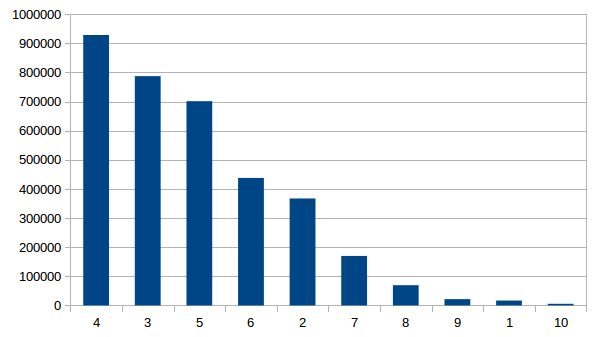
\includegraphics[width=0.48\textwidth]{charts/fig_all_word-length-graph}
\centering
\end{figure}
